% a tikz figure for decision fusion block diagram

\usetikzlibrary{shapes}

\tikzstyle{edata}=[draw,thick,rounded corners,minimum height=1cm,text width=2cm,align=center]
\tikzstyle{data}=[above,text width=1.5cm,align=left]
\tikzstyle{process}=[rectangle,draw,thick,minimum height=1cm,text width=2cm,align=center]
\tikzstyle{fusion}=[rectangle,draw,thick,minimum height=4cm,text width=2cm,align=center]
\tikzstyle{io}=[]

\resizebox{\textwidth}{!}{
\scriptsize
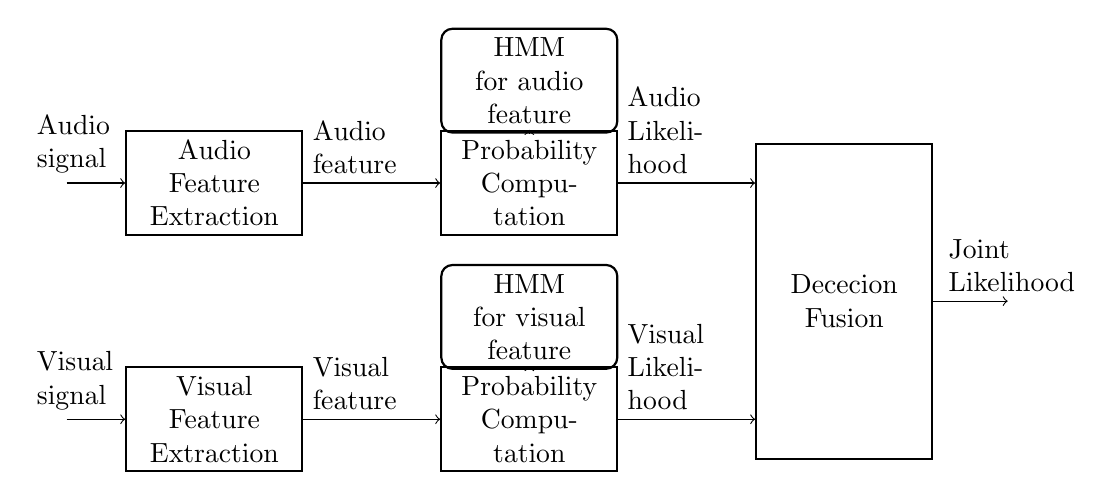
\begin{tikzpicture}
  \node[io] (iv) at (1,0) {};
  \node[process] (pv) at (3,0) {Visual Feature Extraction};
  \node[io] (ia) at (1,3) {};
  \node[process] (pa) at (3,3) {Audio Feature Extraction};
  \node[process] (cv) at (7,0) {Probability Computation};
  \node[process] (ca) at (7,3) {Probability Computation};
  \node[fusion] (df) at (11,1.5) {Dececion Fusion};
  \node[edata] at (7, 1.3) {HMM for visual feature} edge[->] (cv);
  \node[edata] at (7, 4.3) {HMM for audio feature} edge[->] (ca);
  \node[io] (o) at (13.2,1.5) {};

  \draw[->] (iv) -- node[data] {Visual\\ signal} (pv);
  \draw[->] (ia) -- node[data] {Audio\\ signal} (pa);
  \draw[->] (pv) -- node[data] {Visual\\ feature} (cv);
  \draw[->] (pa) -- node[data] {Audio\\ feature} (ca);
  \draw[->] (cv) -- node[data] {Visual Likelihood} (cv -| df.west);
  \draw[->] (ca) -- node[data] {Audio Likelihood} (ca -| df.west);
  \draw[->] (df) -- node[data,pos=1] {Joint\\Likelihood} (o);
\end{tikzpicture}
}

